\documentclass{vldb}
\usepackage{graphicx}
\usepackage{listings}
\usepackage{color}
\usepackage{url}

\begin{document}

\title{CVL: Declarative Spatial Sampling in the RDBMS}

\numberofauthors{1}

\author{
\alignauthor
Pimin Konstantin Kefaloukos, Marcos Vaz Salles \& Martin Zachariasen\\
       \affaddr{Department of Computer Science}\\
       \affaddr{University of Copenhagen}\\
       \email{\{kostas,vmarcos,martinz\}@diku.dk}
}
\date{30 July 1999}

\maketitle

\begin{abstract}
\end{abstract}

% !TEX root = ./cvl.tex
\section{Introduction}

%\marcos{The introduction now reads a bit too generic, and a bit too rich in buzzwords (big data, crowd sourcing). What is the problem that is being addressed?}
%what's the situation

%- why do people need to do cartographic generalization?

%- how do people go about this task today?

%- what is the main related work, and why is it not enough?

Map generalization has a long tradition spanning hundreds of years, and has rightly been considered as much an art as a science~\cite{rieger1993consensus}. The goal of map generalization is to produce a good map at a given scale, which involves both data reduction and choice of graphical symbolization~\cite{brassel1988generalization,gruenreich1985cag}.  In \emph{automated} map generalization this tasks is performed by algorithms on a computer.

In areas such as social networks, factivism and data journalism~\cite{cohen2011journalism,bono,sankaranarayanan2009twitterstand} there is a constant need for visualizing new, narrow and often massive geospatial datasets. For example, a news agency may publish a zoomable map that displays interesting spatial data from a social network. A system for this use case must as a minimum handle big spatial datasets, be able to run without intervention from experts, and complete in a time that works for an environments with tight deadlines. Ideally, the system will allow users to control the important aspects of solutions and reuse existing technology as much as possible.

Spatial data is often stored in a database with powerful spatial extensions installed, so a natural idea is to exploit the processing capabilities of the database to perform map generalization. In this work we present a novel \emph{database integrated} approach which is a complete solution to the data reduction problem while deferring graphical symbolization to a later stage. All operations are performed entirely within the database process, and the result is a spatial database were records are preprocessed for fast execution of subsequent scale-parameterized queries. Essentially a number is assigned to each spatial record which is the lowest zoom-level at which the record should be visible in a zoomable map, which allows for efficient indexing.

Using a \emph{declarative language}, we allow the user to concisely express spatial constraints and an objective function, that are used to compute a multi-scale database from an input database of spatial data. This gives users a large amount of control over the map generalization process, while still being extremely concise.

To our knowledge two significant papers have recently been published that present solutions to the data reduction problem~\cite{nutanong2012multiresolution,sarma2012fusiontables}. While both of these provide good solutions to the data reduction problem, there are distinct and overlapping shortcomings to both of these which are not suffered by our approach.  Both of these approaches support only fixed constraints, while we allow a large class of constraints to be defined by the user. The first paper~\cite{sarma2012fusiontables} seems to indicate that the dataset must fit main memory and requires data to be serialized in and out of the database for processing, none of which is true of our system. The other published approach~\cite{nutanong2012multiresolution} seems to require modifications to the database engine, which is not true of our system. Neither of these previously published systems offer a language for users, but do provide parameterization of the fixed constraints. While~\cite{sarma2012fusiontables} show that there is mathematical support in their approach for several different objective functions, it is not clear how a user would actually express new objectives in a way that is understood by the system. Finally, users can take our implementation and start running it on their own infrastructure using only free, unmodified, open source software.

In this paper, we make the following four contributions:
\begin{enumerate}
\item Define a declarative language, Cartographic Visualization Language (CVL), for generalizing spatial datasets. CVL is designed to be simple and efficient to use for non-cartographers while also allowing for efficient evaluation.

\item Map the generalization problem to the \emph{set multicover problem}, which makes constraints fully pluggable and allows reuse of well-known algorithms.

\item Show how to fully evaluate CVL inside the database; this enables us to reuse basic database technology for data management and scalability. While CVL is designed to compile to a variety of engines, we present here other languages that can run where the data is stored, e.g. SQL or MapReduce.

\item Present experimental results for a variety of real datasets. The results show that the proposed approach has good performance and produces high-quality cartographic generalizations. [Mention GST somewhere here?] 
\end{enumerate}

In Section~\ref{sec:background} we define the multi-scale filtering problem for cartographic generalization. In Section~\ref{sec:cvl:language} we introduce the CVL language. In Section~\ref{sec:optimizationmodel} we introduce the mapping to the set multicover problem, and we revisit algorithms for this problem in Section~\ref{sec:algorithms}. In Section~\ref{sec:implementation} we introduce the compilation procedure, which enables us to run CVL on a relational database backend. Experimental results are presented in Section~\ref{sec:experimental}, and finally related work is summarized in Section~\ref{sec:related}.




% !TEX root = ./ICDE14_conf_full_296.tex
\section{\hl{Selection of Geospatial Data}}
\label{sec:background}

\hl{In the }\emph{\hl{selection problem,}}\hl{ we wish to select the subset of a geospatial dataset to be visualized on a map at a given scale}. Below we define the basic components of the problem, and informally define the associated optimization problem.

\subsection{Geospatial records and weights}
\label{sec:records}

The dataset is assumed to consist of a set of \emph{geospatial records} drawn from a database table. The schema of a geospatial record consists of a \emph{geometry} field (e.g. a point, line or polygon), a \emph{unique ID} field and any number of additional textual and numeric fields, such as ``city name'' and ``population''.

Each record is assigned a \emph{user defined weight} using CVL (see Section~\ref{sec:cvl:language}). \hl{The weight models the importance of a record, with high weight corresponding to great importance}. Any subset of records --- or all records for that matter --- may have the same weight. Therefore, the weights induce a partial order of the records.

\subsection{Zoom levels and map constraints}
\label{sec:constraints}
\hl{For zoomable maps, different subsets of the data should be selected for display at different scales or }\emph{zoom levels}. Let the zoom-levels run from 1 (lowest scale) to $\mathcal{Z}$ (largest scale). On a given zoom level, the map is rendered at a certain pixel resolution. Thus, for a given zoom level, we know the distance in pixels between geospatial locations. This gives rise to two particularly important map constraints~\cite{harrie2007modelling} \hl{when selecting data for a given zoom level}.

Firstly, the \emph{principle of constant information density} implies that the number of records that can be displayed \hl{within an area or a certain pixel size should be bounded}~\cite{topfer1966principles}. Assume that we divide the complete map into cells (or tiles) of, say, 256 x 256 pixels. The \emph{visibility} constraint states that each cell can contain at most $K$ \hl{selected} records, where $K$ is a user-defined parameter~\cite{sarma2012fusiontables}.

Secondly, records cannot be too close to each other in the map --- otherwise the user will not be able to \hl{clearly distinguish between them}. The \emph{proximity} constraint states that every pair of visible records must be separated by at least $d$ pixels, where $d$ is a user defined parameter.

In addition to these constraints that must hold separately for each zoom level, there are constraints that must hold across zoom levels. A particularly important constraint is the \emph{zoom-consistency} constraint, which states that when a record is filtered out at a given scale, it should also be filtered out at all \emph{lower} scales~\cite{sarma2012fusiontables}. When a user zooms out on a map, records can only disappear --- not reappear.

Apart from the zoom-consistency constraint, \hl{CVL supports constraints based on }\emph{simple measures}\hl{ that are }\emph{satisfiable by selection} (see Section~\ref{sec:cvl:language}).\hl{ A simple measure is a function that maps a set of records to a scalar value. A constraint is violated if the measure exceeds a threshold. A constraint is satisfiable by selection if we can }\emph{always}\hl{ satisfy it by simply deleting an appropriate subset of the records. Both the visibility and proximity constraints respect these restrictions. However, we cannot model constraints that have complex measures or cannot be satisfied by using selection alone, such as }\emph{topology}\hl{ and }\emph{spatial distribution}\hl{ constraints. We leave these classes of constraints to future work.}

\subsection{\hl{Conflicts}}
\label{sec:conflicts}

\hl{Constraints such as visibility or proximity can be modeled using the notion of }\emph{conflicts}. \hl{A conflict is a set of records that cannot all be selected without violating the constraint}.

\hl{For the visibility constraint, there is a conflict generated for every cell that contains more than $K$ records. For the proximity constraint, there is a conflict generated for each pair of records that is less than $d$ pixels apart (see Figure}~\ref{fig:proximity:conflict}\hl{)}. A record can be in several \hl{conflicts}, which is the case for point $p$ in the example shown in the figure. \hl{A solution to the selection problem is }\emph{feasible}\hl{ if there are no conflicts}.

\begin{figure}[htbp]
\begin{center}
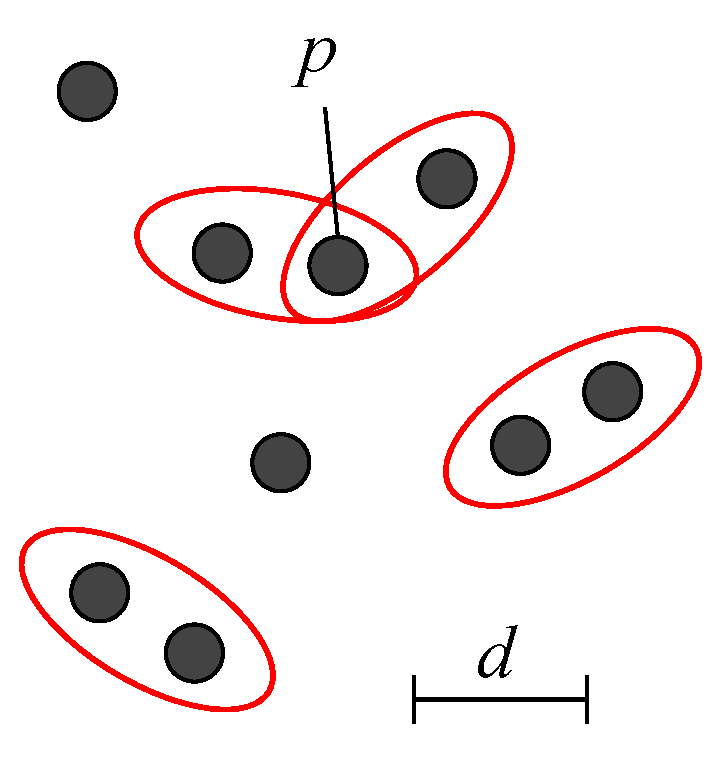
\includegraphics[scale=.3]{figs/cvl_proximity_conflicts.pdf}
\caption{Conflicts generated by the proximity constraint for distance $d$. Notice that point $p$ is a member of more than one \hl{conflict}.}
\label{fig:proximity:conflict}
\end{center}
\vspace*{-4ex}
\end{figure}

Consider a \hl{conflict involving} $k_1$ records, where at most $k_2$ of these records can be selected (where $k_1 > k_2$). Then it is equivalent to state that at least $\lambda = k_1 - k_2$ of these records must be \emph{deleted}. In the mathematical formulation of the problem in Section~\ref{sec:optimizationmodel}, we will use this alternative way to formulate \hl{conflicts}.

\subsection{\hl{Selection as an optimization problem}}
\label{sec:filtering}
\hl{The notion of conflicts is used to define the feasibility of solutions to the selection problem. This should be accompanied by a way to discriminate between solutions. Assigning an importance measure to each record, namely the record weights, intuitively allows us to measure the ``loss of importance'' due to records that are deleted.} 

\hl{In the optimization version of the problem, we seek the feasible solution that minimizes the aggregate weight of records that are deleted. In Section}~\ref{sec:optimizationmodel}\hl{, we present a mathematical formulation of the selection optimization problem}.

\hl{For a zoomable map with }$\mathcal{Z}$\hl{ zoom levels, we are interested in finding $\mathcal{Z}$ solutions to the selection problem, one for each zoom level }$i \in \lbrack 1, \mathcal{Z} \rbrack$. \hl{We call this problem the }\emph{multi-scale selection problem}. \hl{To control the way in which we compute these solutions, we use an algorithmic framework known as the }\emph{ladder} approach~\cite{foerster2010challenges}. \hl{This is a recursive approach, where the output of selection at large scale is used as input to selection at a smaller scale. This means that the zoom-consistency constraint }(Section~\ref{sec:constraints})\hl{ is automatically satisfied}.

\hl{The ladder approach is not appropriate for all use cases. For example, when regional labels are modeled as geospatial records, e.g., the label ``Europe'', we may wish to show a record only on intermediate zoom levels, violating zoom consistency. Handling these use cases would require an alternative formulation, e.g., following the }\emph{star} \hl{approach}~\cite{foerster2010challenges}. \hl{This is an interesting avenue for future work}.  

% should be visible mostly on the intermediate zoom levels, the }\emph{star} approach~\cite{foerster2010challenges}\hl{ would be better. This is a limitation of the work presented in this paper.}







% !TEX root = ./cvl.tex
\section{Model}
Not a word about SQL here. Here the various constraints are mentioned and illustrated using nice figures. The hitting set problem is mentioned. The ranking of records is mentioned.

% !TEX root = ./cvl.tex

\section{Implementation}
\label{sec:implementation}

In this section, we present how our implementation makes use of in-database execution to provide scalability and engine reuse for CVL (Section~\ref{sec:implementation:indatabase}). In addition, we discuss a number of extensions to CVL that we found to be useful for practical applications (Section~\ref{sec:implementation:extensions}). 

\subsection{In-Database Execution}
\label{sec:implementation:indatabase}

\minisec{Overview}
Since CVL is declarative, and CVL constraints are already expressed in SQL, it is natural to attempt to reuse as much existing DBMS technology as possible to execute CVL. Figure~\ref{fig:indatabase} shows how CVL is compiled for execution in a relational DBMS, which acts as the language runtime. The output of the CVL compiler is a database script for the target host, containing both SQL and stored procedures, and following the algorithmic framework of Figure~\ref{fig:algorithmic-framework}. The script is pushed down to the database engine, and operates against the appropriate input data stored in the system. This strategy offers us two main advantages:

\begin{enumerate}

\item Since all code is pushed down and both input and output reside in the database, we do not need to transfer any data outside of the database engine. This co-location of code and data is a significant advantage for large datasets.

\item By expressing as much as possible of the generated code in SQL, we can reuse decades of optimizations built into database engines, especially for geospatial data~\cite{Guttman1984:RTree,Hellerstein1995:GiST}. This opens up many opportunities, such as automatic optimization, parallelism, and selection of specialized algorithms and indexes.  

\end{enumerate} 

While the general strategy of compiling declarative languages to SQL has been pursued in other contexts, e.g., for XQuery~\cite{pathfinder} and LINQ~\cite{ferry}, our context poses a particular challenge of integrating the language with algorithmic solvers inside the database. 

\begin{figure}[htbp]
\begin{center}
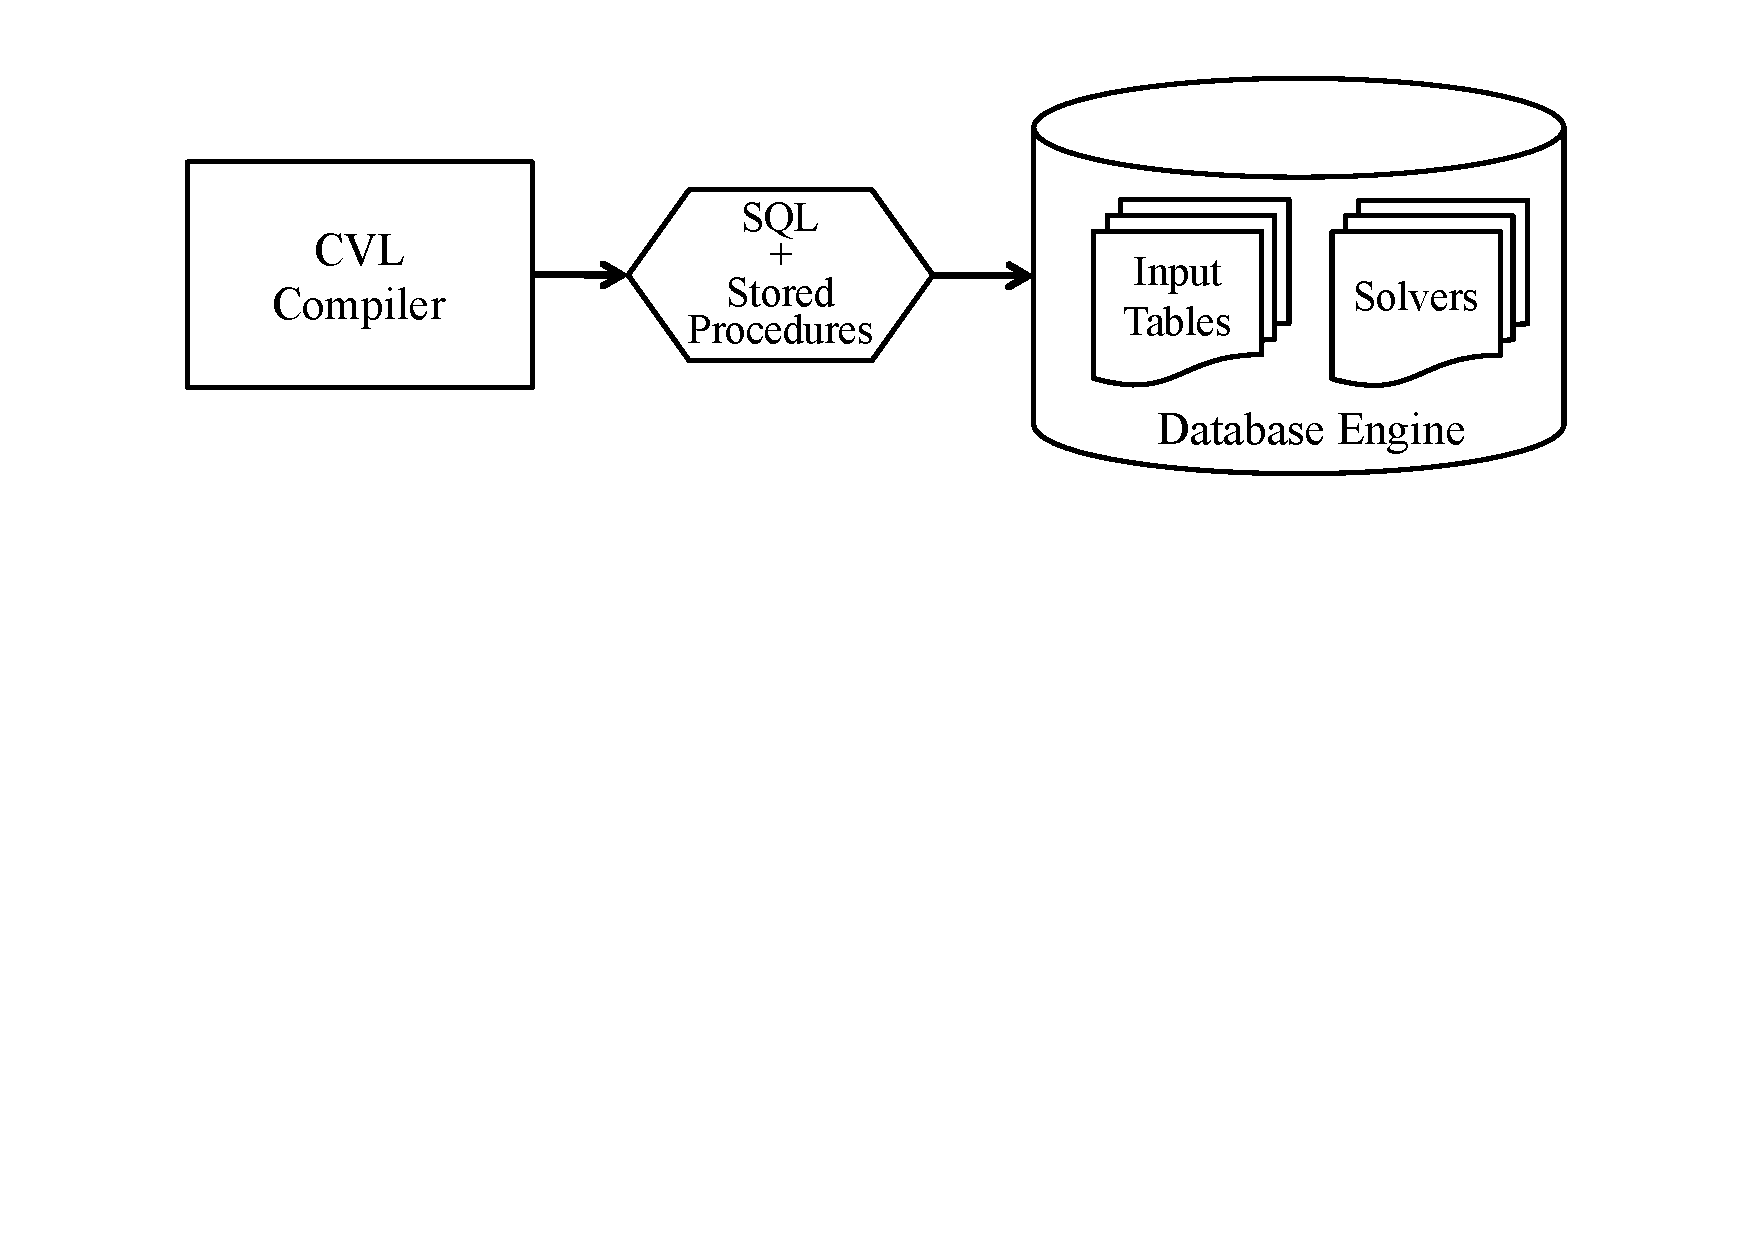
\includegraphics[scale=.35,viewport=400 375 450 550]{figs/indatabase-execution.pdf}
\caption{CVL and in-database execution.}
\label{fig:indatabase}
\end{center}
\end{figure}

\minisec{Solvers}
In Section~\ref{sec:algorithms}, we have presented two different algorithmic approaches for solving CVL generalizations: static greedy (SGA) and LP-based greedy (LPGA). We now show how to express each of these approaches in SQL along with stored procedures. 

SGA is the simplest algorithm, and recall that it operates independently on the conflicts generated by each constraint. Suppose the conflicts $\bar{C}$ generated by the active constraints are stored in a \emph{conflicts} table. Then for conflict set $c \in \bar{C}$, SGA is tantamount to the query:

\begin{lstlisting}
SELECT rid
FROM (
  SELECT ROW_NUMBER() 
         OVER (PARTITION BY cid
               ORDER BY cvl_rank) AS r,
         rid, cvl_rank, lambda_c
  FROM conflicts) h
WHERE h.r <= h.lambda_c
\end{lstlisting}

For each conflict set $c$, we order records by rank, and ensure that we pick at least $\lambda_c$ records. The declarative formulation allows us to reuse optimized sorting code in the database engine for execution.

LPGA solves a linear programming relaxation of the set multicover problem. We express LPGA by a stored procedure. The procedure accesses the conflicts for the constraints via SQL, constructs an appropriate LP, and then calls into an LP solver library~\cite{cvxopt}. Since the solver library does not use built-in database optimizations, this execution strategy for LPGA only leverages the first advantage of data and code co-location listed above.

Finally, note that the code for finding conflict sets is already expressed in SQL by the user for each constraint. As a consequence, this user code can make use of all built-in database optimizations available in the target engine.

%\minisec{CVL runtime functions}
%In the definition of the visibility constraint in Section~\ref{sec:create:constraint:statement} we reference two stored procedures in the CVL runtime library, \texttt{CVL\_PointHash} and \texttt{CVL\_WebMercatorCells}. These functions are implemented in SQL and make use of the spatial extension of the database~\cite{postgis}.

%The procedure \texttt{CVL\_PointHash} uses a call to \texttt{ST\_GeoHash} to implement an injective mapping from points to strings. The GeoHash algorithm corresponds to a Z-order curve, and we exploit this for uniquely naming tiles when evaluating the visibility constraint, i.e. finding tiles with more than $K$ records.

%The \texttt{CVL\_WebMercatorCells} function maps a geometry at a given zoom-level to centroids of all intersected tiles (on that zoom-level). We experimented with several ways to do this for general geometries (points, line segments, polygons) and found that rasterizing the geometry (using the function \texttt{ST\_AsRaster} in the spatial extension of the database) and iterating over the indices was the fastest for general geometries. For point records it is significantly faster to use the standard transformation function \texttt{ST\_SnapToGrid}.

%An improvement to \texttt{CVL\_WebMercatorCells} that we did not have time to implement is to compute tiles as quad-keys on the highest level only. Tile identifiers for lower levels are easily computed by taking prefixes of the quad-keys. This approach only benefits the running time when using constraints that are tile-based.

\subsection{Extensions}
\label{sec:implementation:extensions}

When designing CVL, we realized a number of our interesting use cases for the language that we had not initially considered. This realization, along with our implementation experience of CVL use cases, led us to a set of extensions over the core language targeted at improving convenience of use. We present these extensions below.

\minisec{Partitioning and Merging Datasets} 
A single input table may contain geospatial objects of different classes, e.g., roads and points of interest. When this is the case, users often wish to generalize some of these classes of objects independently, but obtain a single result map. While this can be done by merging the results of multiple GENERALIZE statements, we found it useful to add syntactic sugar to support this case. We extend the GENERALIZE statement with PARTITION BY and MERGE PARTITIONS clauses. PARTITION BY allows us to effectively segregate the input into multiple independent sets. MERGE PARTITIONS combines a few of these sets back together before providing them as input to generalization. For example, assume a \emph{geo\_objects} table contains highways, roads, restaurants, and hotels, tagged by a \emph{type} attribute. We could then generalize \emph{geo\_objects} as follows:

\begin{lstlisting}
GENERALIZE  geo_objects
TO network_and_poi_map
...
PARTITION BY type
MERGE PARTITIONS 'restaurant', 'hotel' 
              AS 'poi'
... 
\end{lstlisting}

In the example, we overlay independent generalizations of highways, roads, and points of interest into a single map. However, restaurants and hotels are generalized as a single input set.  

\minisec{Forced and All-or-Nothing Visualization}
Intuitively, constraints let users specify what is \emph{not} allowed in a given map, by forbidding the existence of conflicts. However, users also find helpful to control certain behaviors that \emph{must} occur in their map. We extended the GENERALIZE statement with support for two types of behaviors: (1)~the ability to mandate a minimum zoom level for a particular partition of the input, and (2)~the ability to force that either all or none of the objects of a given partition be displayed. For example, a user may wish to specify that highways must only appear at zoom level 10 or lower in their map. In addition, for consistency, either the whole highway skeleton is displayed or no highways should show up. To achieve this goal, we extend the GENERALIZE statement by a FORCE clause with MIN LEVEL and ALLORNOTHING specifiers. Continuing the example above:

\begin{lstlisting}
...
FORCE MIN LEVEL 10 ALLORNOTHING FOR 'highway'
... 
\end{lstlisting}

In the evaluation of CVL, the minimum level specifier controls what data is given as input for a zoom level. The all-or-nothing specifier, on the other hand, controls filtering of the output of the level generalization process. If the specifier is present, all records of a partition are eliminated if any record from the partition input is not present in the output. By filtering output, we ensure that the result also respects all other constraints specified by the user. 

%\minisec{Set up and Tear Down for Constraints}   
%Map constraints can exhibit significant complexity. Since a constraint is expressed as a single SELECT statement, it is often helpful to be able to refer to temporary tables in its formulation. We have thus extended the CREATE CONSTRAINT statement to include two additional clauses: WITH SETUP and WITH TEARDOWN. The former allows a user-defined SQL statement to be executed in advance of the constraint evaluation, creating any supporting tables for the evaluation of the constraint. The latter specifies user-defined cleanup code. Note that since constraints are evaluated independently at each zoom level, the set-up and tear-down clauses are evaluated before and after the constraint SQL at each zoom level.       
%\marcos{Move necessary information from paragraph above to Language section, and remove paragraph after that.}

%
% MVS: We can probably get away with not showing the syntax below. 
%
%\begin{lstlisting}
%CREATE CONSTRAINT C1 
%AS NOT EXISTS
% (SELECT cid, rid, minhits
%  FROM {more SQL})
%WITH SETUP
% {user-defined SQL}
%WITH CLEANUP
% {user-defined SQL}
%\end{lstlisting}



% !TEX root = ./cvl.tex
\section{Results}
Show performance, scalability and quality.

% !TEX root = ./cvl.tex
\section{Related work}
\label{sec:related}
\marcos{One should make sure to include the items below.}

Basic reference set:

\begin{itemize}

\item Fusion Tables~\cite{sarma2012fusiontables}. 
% zoom consistency, adjacency, visibility; not general constraints. // different types of objectives, but no declarative interface and integration with standard database technology.

\item Summary and most important references from cartographic generalization survey.

\item Reverse data management vision~\cite{meliou2011reverse}

\end{itemize}

Additional references:

\begin{itemize}

\item In-database processing: briefly repeat argument with Pathfinder and Ferry (As we mentioned earlier,...). Increasingly, relational are incorporating whole programming language interpreters and support for spatial data structures~\cite{Blakeley2008:DotNET}. Then also cite MADLib work~\cite{hellerstein12madlib} as well as Ordonez~\cite{ordonez10udf}. But: direct SQL and not higher-level DSL leveraging SQL + analytics / statistics and not spatial.  

\item Say something about how you actually serve the map after it is built with our framework (e.g., the usual references in linearization)~\cite{hilbert1891ueber}.

\item ...

\marcos{Still performing scan of recent literature, just in case.}

\item if it fits, reverse / symbolic query processing.

\end{itemize}

\martin{We should mention that the dynamic greedy algorithm would have improved the running time compared to the LP-based greedy algorithm, while achieving good quality~\cite{rajagopalan1998primal}.}


% !TEX root = ./cvl.tex
\section{Conclusion}


% The following two commands are all you need in the
% initial runs of your .tex file to
% produce the bibliography for the citations in your paper.
\bibliographystyle{abbrv}
\bibliography{cvl}  % gvl.bib is the name of the Bibliography in this case
% You must have a proper ".bib" file
%  and remember to run:
% latex bibtex latex latex
% to resolve all references

\subsection{References}
Generated by bibtex from your ~.bib file.  Run latex,
then bibtex, then latex twice (to resolve references)
to create the ~.bbl file.  Insert that ~.bbl file into
the .tex source file and comment out
the command \texttt{{\char'134}thebibliography}.


\end{document}
